\section{Integration}
\label{sec:integration}

This section describes how we integrate the components described in section \ref{sec:design}. The section is divided according the online and offline parts of the \gls{rec}.

\begin{description}
\item[Offline learning] In this part the systems uses the stored histories of user behavior to compute the \gls{llr} ratios of the \gls{coocc} among items. Then it updates all items in the in the NoSQL database/search engine Apache Solr. We use similar items as indices and store the \gls{llr} ratios from the previous step as payloads. This task takes serveral minutes but the duration does not impact the user experience hence it can be executed overnight. 
\item[Online logging and recommendation] The online part of the system records user activities used in the similarity analisis and create personalized \gls{topn} if requested. If it receices a requerst for a recommendation list it constructs a query from the user history $h_u$. Then it uses the query to get a ranked list of items that are likely appealing to the user $u$. It removes all item's the user already knows and present the list as recommendation. In order to a  provide smooth user experience the top-N recommendation task should not take longer than a second.
\end{description}

To store the user's activity we used a sqlite3 database because it's easy to deploy in a development environment and we can use existing interfaces to from Java and Python to update and retrieve data. 

First we insert a document for every item into Solr. The documents contain the metadata like (title, genre, tags, etc). The offline learning step will only update the indicator fields for every item.

\subsection{Offline learning}
\label{sec:offline}

\begin{figure}
\centering
\begin{tikzpicture}[node distance=20mm,
data/.style={
rectangle,
draw,
thin,
minimum height=3.5em
},
to/.style={->,>=stealth',shorten >=1pt,semithick,font=\footnotesize},]

\node (history) [data,align=left] {user actions\\database};
\node (spark) [data,right of=history,node distance=50mm, align=left] {Mahout's \\\verb|RowSimilarityJob|};
\node (solr) [data,below of=spark,node distance=3cm] {Apache Solr};
\draw[to] (history) -- node[midway,above]{user actions} (spark);
\draw[to] (spark) -- node[midway,right] {similarity indicators} (solr);
\end{tikzpicture}
\caption{The offline learning part uses user log files stored in a sqlite3 database to compute the similarities with Mahout's {\ttfamily RowSimilarityJob}. The result is loaded into Solr.}
\label{fig:offline}
\end{figure}

The offline learning part is done in three steps.

\begin{enumerate}
\item Read the recorded \glspl{useraction} from a sqlite3 database and convert it as required by \verb|RowSimilarityJob|.
\item Generate \glspl{indicator} with Mahout's \verb|RowSimilarityJob| that connects to a Apache Spark server.
\item Use the output of \verb|RowSimilarityJob| to update the indicator fields of all items stored in Solr.
\end{enumerate}

The computation of similarities and update of Solr involves a lot transforming data from one format to another. We have implemented a command line tool, \verb|updatesearchengine|, that executes all three steps. 

\subsection{Online recommendation}
\label{sec:online}

In our demo application the user interacts with a web GUI in a web brower. 
\subsubsection{Retrieve recommendation}

In order to produce recommendations we compose a Solr query from the user history. The user history is stored in the web log. The web server sends this query to Solr. Solr responds with a ranked result set. The web server then formats the response from Solr and sends a list of recommended items to the user.

\begin{figure}
\centering
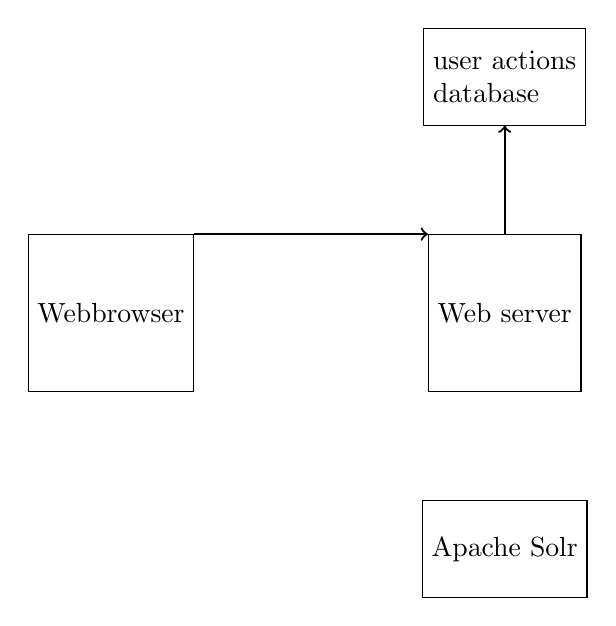
\begin{tikzpicture}[node distance=20mm,thick,
data/.style={
rectangle,
draw,
thin,
minimum height=3.5em
},
]

\node (web) [data, minimum height=2cm] {Web server};
\node (log) [data,above of = web,align=left,node distance=30mm] {user actions\\database};
\node (browser) [data,left of=web,node distance=50mm,minimum height=2cm] {Webbrowser};
\node (solr) [data,below of=web,node distance=30mm] {Apache Solr};
\draw[->] ([yshift=1 cm]browser.east) --  ([yshift=1 cm]web.west);
\draw[->] (web) -- (log);
\end{tikzpicture}
\caption{The web server sends this query to Solr. Solr responds with a ranked result set.}
\end{figure}
%-- node[midway,above] {post user actions}